\documentclass[letter,12pt]{article}
\usepackage{fancyhdr}
\usepackage{amsmath}
\usepackage{amssymb}
\usepackage{bm}
\usepackage{synttree}
% \usepackage[margin=1in]{geometry}
\usepackage{graphicx}
\pagestyle{fancy}
\lhead{Jesse Mu}
\rhead{CSCI339 Term Project}

\begin{document}

\title{How Are You Feeling? Analyzing Twitter User Mood with Naive Bayes
Sentiment Analysis}
\date{December 12, 2014}
\author{Jesse Mu}
\maketitle

\section{Background}

Sentiment analysis is a relatively new subset in the relatively new field of
machine learning but has since found significant research interest and
application in business analytics. Social networking site
Twitter\footnote{https://www.twitter.com/} has been identified as a key data
source to assist in sentiment analysis study. Given its status as one of the
biggest social networking sites in the world and its focus on trending topics
and discussion using hashtags, Twitter users' tweets represent a massive,
real-time snapshot of much of the world's opinions on countless topics---one of
the most valuable and accessible resources of its kind.

Sentiment analysis is an example of a machine learning classification problem.
As such, work in the field draws from standard classification models in the
literature (e.g. Support Vector Machines, Maximum Entropy Models, Naive Bayes
Classifiers) as applied to text classification \cite{pang02}. The fundamental
challenge of sentiment analysis is building a computer program that is able to
``learn'' from given data to generalize and form conclusions about new, unseen
examples. This can be successfully approached by the more standard supervised
(training data labeled with sentiment) approach or an unsupervised, lexical
(unlabeled training data) approach \cite{turney02}.

The classical application of sentiment analysis is opinion mining of movie
reviews, but the recent and dramatic surge in popularity of Twitter has
resulted in substantial research interest in the potential for usage of English
tweets as a corpus. Among the reasons for the usage of Twitter for sentiment
analysis provided by Pak and Paroubek \cite{pak10} are the inherent
subjectivity of social microblogging platforms, a large and incredibly varied
userbase, and potential for an ``arbitrarily large'' amounts of data.

When compared to other opinion mining tasks, sentiment analysis with a Twitter
corpus stands out because of the linguistic properties of its training
``documents.'' Tweets are incredibly short messages, with a 140-character
maximum limit, and encourage a fast, fundamentally electronic method of
communication. The casual, spontaneous, and compressed nature of the service
presents interesting and unique challenges. Specifically, feature extraction
has been the distinguishing area of research when dealing with tweets, as
researches encounter microblogging-specific problems including the usage of
emoticons, abbrevations, sarcasm, and the sheer brevity of the information
given.

Twitter sentiment analysis is not limited to the academic space. A critical
aspect of many companies' success is the successful monitoring and analysis of
subjective information on a product through social media, and sentiment
analysis on microblogging platforms plays a pivotal role. Because of the
uniqueness of its content, the issue of Twitter sentiment analysis has led
several companies to identify the problem as unique from standard sentiment
analysis programs, and some text analysis companies such as Datumbox employ a
separate Twitter analysis classification algorithm in addition to the
traditional classifier. In addition to Datumbox's API, several other commercial
services exist specifically for the sentiment analysis of English tweets. Many
o them are at least partially free to use, including
Sentiment140\footnote{http://www.sentiment140.com/},
Streamcrab\footnote{http://www.streamcrab.com/}, and
Semantria\footnote{https://semantria.com/}. A well-performing sentiment
analysis algorithm is a valuable asset, which motivates several of these
companies to keep their code closed-source, like Sentiment140 and Semantria.

\section{Problem Formulation}

\subsection{Corpus}
Because Twitter sentiment analysis is a relatively new
problem, there do not exist many good sources of labeled data for supervised
learning tasks. It is possible to train a classifier based on standard
sentiment data, e.g. from well-known movie review datasets, but the unique
terminology and writing style of tweets demands a native training corpus.

Previous papers have used smaller training sets such as the 2013 SemEval
corpus\footnote{http://www.cs.york.ac.uk/semeval-2013/task2/} ($\sim$9000
tweets) and the Sanders Analytics training
corpus\footnote{http://www.sananalytics.com/lab/twitter-sentiment/} ($\sim$5500
tweets) For this project, training data was taken from the Stanford
University-associated online tool Sentiment140 mentioned previously, which
provides a much larger corpus of 1,600,000 labeled tweets.

The sheer volume of tweets made available by Sentiment140 is due to the
automatic collection of tweets based on a simplifying assumption: any tweet
with positive emoticons (\texttt{:D}, \texttt{:)}, \texttt{=)}, etc) is labeled
as a positive tweet, and any tweet with negative emoticons (\texttt{:(},
\texttt{D:}, \texttt{=(}) is labeled as negative \cite{go09}. Intuitively, this
assumption seems reasonably valid; due to the short nature of tweets, those
with a positive emoticon are quite unlikely to have another negative emoticon
resulting in an overall negative sentiment. Of course, there are certainly
cases where this assumption fails, such as the usage of sarcasm and quoting.
Another disadvantage of this data set is that it makes no qualification based
on language; tweets of all languages are accepted, which decreases accuracy of
a solely English-based classifier. However, the sheer volume of this data set
outweighs other data sets by orders of magnitude and smooths out most anomalies.

\subsection{Naive Bayes}

Because the main area of focus in Twitter opinion
mining is good, reliable text preprocessing and feature extraction, multiple
classifiers were not considered. The best classification algorithm for
sentiment analysis tasks is disputed, and Go et al. \cite{go09} reports that
the optimal model is unclear, but one common, well-performing model suggested
by Gamallo \cite{gamallo14}, Narayanan \cite{narayanan13} and Pak \cite{pak10}
and used commercially by companies like Datumbox is the Naive Bayes classifier.

For each document $d$, Naive Bayes attempts to assign the class $c$ to $d$
where

\begin{equation}
  c = \max_{c_i} P(c_i | d)
\end{equation}

Bayes' Rule shows us that for each $c_i$, $P(c_i | d)$ is equivalent to

\begin{equation}
  P(c_i|d) = \frac{P(d | c_i)P(c_i)}{P(d)}.
\end{equation}

The Naive Bayes algorithm then makes several simplifying assumptions. Because
for each document $d$, $P(d)$ is constant, it can simply be ignored without
consequence. Furthermore, $P(d | c_i)$ is calculated by considering the
features of document $d$, $x$, where $x_1 x_2 x_3\dots x_i$ are individual
features. The Naive Bayes model \emph{naively} assumes independence of these
features, giving the simplified model

\begin{equation}
  P(c_j | d) = P(c_j) \prod P(x_i | c_j).
\end{equation}

Depending on whether or not we have a prior belief about the distribution of
classes $P(c_j)$, the Naive Bayes model can either take this prior belief into
account or learn from the training data class occurrences. If all classes are
equally likely, the term $P(c_j)$ becomes irrelevant.

There are many advantages of the Naive Bayes classifier, although of course
several disadvantages. Perhaps the benefit most tangible to this project is the
speed and simplicity of the Naive Bayes algorithm, which requires considerably
less time and memory consumption than similar classification algorithms such as
SVM and ensemble learning methods \cite{huang03}. Considering feature selection
is paramount, a fast algorithm allows for rapid experimentation and
prototyping, which makes detailed statistical analysis substantially easier.
Despite its arguably oversimplifying assumptions, Naive Bayes is uniquely good
at dealing with discrete text classification features, since more advanced
feature selection techniques such as n-grams can compensate. Again, although
disputed, Naive Bayes has been shown to outperform other algorithms in this
task \cite{narayanan13,pak10}.

Concerning disadvantages, one main issue with the Naive Bayes classifier is the
lack of a reliable confidence metric when making decisions on new documents.
Although the Naive Bayes classifier can output the probability it estimates for
each class, the classifier tends to be overconfident \cite{rennie01}. This can
pose problems when considering the web application in Section~\ref{sec:web}

There are two main variants of the Naive Bayes classifier used for
discrete data, Bernoulli and Multinomial, which will be discussed further.

\section{Technologies}

The full source code for this project is open-source and available on GitHub at the following
URL:
https://github.com/jayelm/TwitterSA.

The code is written exclusively in Python, selected primarily due to software
package availability. Text classification code uses the popular
scikit-learn\footnote{http://scikit-learn.org/stable/} machine learning library
which is built on the numpy\footnote{http://www.numpy.org/} and
scipy\footnote{http://www.scipy.org/} scientific computing stack. The result is
a heavily optimized machine learning library that retains the familiar and
intuitive Python syntax while resorting to C bindings and optimizations when
necessary for speed. It also incorporates many useful machine learning
utilities to help automate feature extraction, pipelining, and evaluation.

The web application uses the web framework
Flask\footnote{http://flask.pocoo.org/}, and incorporates the scikit classifier
module written for this project. Flask was chosen due to its minimalism, which
suited the small project at hand; as a microframework, an entire web
application can be written in only a few files, which is ideal for this
project's small, single-use goal.

The cloud hosting service Heroku is used to host the web application. A
development version is running at http://twittersa.herokuapp.com/.

There are also several utility scripts included in the project, written with
Python and Shell, which assist in data sanitization and scraping.

\section{Classifier Evaluation}

The biggest portion of this project was the one specifically concerned with the
natural language processing task at hand, and evaluation was integral to the
development of my classification script and classifiers. Specifically, my goal
was to consider several factors of a Naive Bayes classifier to identify a
configuration most suitable for a production environment. To that end, I first
and foremost attempted to maximize classification accuracy on test sets, while
keeping in mind other important factors like portability (running time, memory
constraints) and other metrics.

\subsection{Preprocessing and Feature Vectorization}

\subsubsection{Preprocessing}

Preprocessing refers to the regularization and normalization of documents to
reduce extraneous document information like punctuation, stopwords, etc. in an
attempt to eliminate the extraction of ``noisy'' features that can decrease
accuracy and performance.

For this task, I created a \texttt{preprocess} function in
\texttt{classifiers.py} that sanitized the document input. After tokenizing the
input with NLTK's \texttt{word\_tokenizer} method (more robust than scikit's),
I implemented the following steps common in most text preprocessing
implementations:

\begin{itemize}
  \item Make all words lowercase.
  \item Decode strings into unicode literals.
  \item Stem each word with the NLTK Porter Stemmer.
  \item Remove punctuation, including Twitter-specific \texttt{@} signs
    (``mentions''), \texttt{\#} signs (``hashtags''), and URL symbols.
\end{itemize}

There are also other issues unique to the language of Tweets that must
be dealt with appropriately. Specifically, this includes the following
implemented steps:

\begin{itemize}
  \item Expanding acronyms (lol, wtf, lmao, etc) using a list of slang words
    from http://www.noslang.com/.
    \begin{itemize}
      \item Since Noslang provides their dictionary freely on the website, but
        not in a computerized format, this required me to create the utility script
        \texttt{util/noslang\_scraper.py}, which visits every page on the
        Noslang website, converting it into a Python dictionary, and
        serializing it.
    \end{itemize}
  \item Removing the occurrences of two-or-more repeated characters to just
    two characters
    \begin{itemize}
      \item E.g. ``cooool'' $\rightarrow$ ``cool'', ``crazyyy'' $\rightarrow$
        ``crazyy''
      \item Duplicate characters cannot completely be removed since it's too
        difficult to know when letters are duplicated due to the correct
        spelling of a word (e.g. ``cool'') or emphasis (``crazyy''). Still,
        partial reduction is better than no reduction, and there may be value
        in differentiating between normal and emphasized uses of words.
    \end{itemize}
\end{itemize}

After the text has been preprocessed, each document must be converted into a
numerical vector to be processed efficiently by a classification algorithm.

\subsubsection{The Bag-Of-Words Model}
\label{ssub:the_bag_of_words_model}

The most commonly used feature vectorization technique when dealing with text
data is the bag-of-words model, which represents each document in a corpus as
the unordered bag of its words.

Specifically, for a training corpus that contains
$n$ globally unique words, a unique numerical index is assigned to each word, 0
through $n - 1$. Once this global tally of words is created, either with a
dictionary or by usage of a hash function, each document $d$ is represented by
a feature vector $x \in \mathbb{R}^n$, where each element $x_n$ stores the
occurrence count of the $n$th word in the given document.

This model works very well when used in tandem with a Naive Bayes classifier,
since such a classifier assumes independence of features and the bag-of-words
model similarly doesn't keep track of word ordering.

Feature vectors created using the bag-of-words method can either be discrete
counts or binary presence attributes, and results in different types of Naive
Bayes classifiers that are discussed in Section~\ref{sub:initial_evaluation}.

Scikit-learn provides the \texttt{CountVectorizer} class for keeping track of
the features and vectorizing a set of data. There are many feature extraction
parameters that can be fine-tuned to produce better performance.

\subsubsection{Laplace Smoothing}
\label{ssub:laplace_smoothing}

\subsection{Initial Evaluation: Bernoulli versus Multinomial Naive Bayes}
\label{sub:initial_evaluation}

There are two main types of Naive Bayes classifiers that handle discrete data,
and they make different assumptions about the probability distribution
underlying the data. The first is the Multinomial Naive Bayes algorithm, which
makes classification decisions assuming the features follow a multinomial
(polynomial) distribution, while the second is the Bernoulli Naive Bayes, which
makes classification decisions based on the Bernoulli (binary) probability
distribution. The main difference between the two is that the Multinomial Naive
Bayes considers the count of occurrences of a given word, rather than just its
presence. On the other hand, the Bernoulli Naive Bayes model works only with
binary features---it considers only the presence of given words. Scikit-learn
provides two classes, \texttt{MultinomialNB} and \texttt{BernoulliNB} that
implement these classifiers. Non-binary data given to a \texttt{BernoulliNB}
instance is binarized and treated like a binary distribution.

One imporant decision to make before continuing with analysis is whether to use
the Bernoulli or the Multinomial distribution. Using a standard bag-of-words
approach with my preprocessing function, figure ? shows both the accuracy and
$F$-score performance metrics for Bernoulli and Multinomial Naive Bayes
classifiers based on varying training sets.

\begin{figure}[h]
  \centering
  \includegraphics[width=0.8\linewidth]{name.ext}
  \caption{Name}
  \label{fig:name}
\end{figure}

\subsection{Improving Classification Accuracy}

\subsubsection{N-grams}
\label{ssub:n_grams}

\subsubsection{Reducing features: select $k$-best}
\label{ssub:reducing_features_select_k_best}

% Use the graph you had before

\subsubsection{Variance Threshold Feature Removal}
\label{ssub:variance_threshold_feature_removal}

% Do some tests

\subsubsection{Term Inverse, Inverse Document Frequency Selection}
\label{ssub:term_inverse_inverse_document_frequency_selection}

% Do some tests

\subsubsection{More Data - Diminishing Returns}
\label{ssub:more_data}


\section{Building the Web App}
\label{sec:web}

\subsection{Backend}

As previously mentioned, the web application was written in
Flask, and simply includes an index page, a user endpoint page, and an error
page. Most of the code is included in \texttt{TwitterSA.py}. When submitting a
request to the \texttt{/search?q=<USER-ID>} endpoint, the user function takes
the supplied Twitter username and attempts to get historical tweets associated
with that user by calling the \texttt{statuses/user\_timeline} Twitter API
endpoint. If no tweets are found, either because the user does not exist or the
timeline is private, an error page is shown.

How many tweets the application gets is dependent on the
\texttt{USER\_API\_CALLS} global variable set in \texttt{TwitterSA.py}. The API
enforces a limit of 200 tweets per user timeline call, and keeps a maximum
of up to 3200 tweets of historical data. Thus, this variable can be anywhere
from 1 to 16, and will attempt to get as many tweets as possible given the API
call limit.

The \texttt{status/user\_timeline} API endpoint is rate-limited to 300 requests
per minute for application-level authentication, so increasing
\texttt{USER\_API\_CALLS} results in quicker exhaustion of the rate allowance.
It is currently set at 2. The application currently uses a singular set of
Twitter API keys from an application registered at dev.twitter.com, since I do
not anticipate usage to be high enough such that the rate limit actually limits
usage of the application.

After tweets are collected, they are sorted by date and put into histogram-like
bins. Depending on the frequency of tweets, they are put into either weekly or
monthly time intervals. Then, the production classifier specified from
\texttt{sentiment/classifiers.py} predicts the sentiment for each tweet,
returning an array of \texttt{TweetSentiment} objects. The average sentiment
for each time interval is calculated, and transformed into a JSON-like object
that will be used for display by the frontend. Both this object and a list of
the original tweets are passed to the HTML view using the jinja2 templating
engine.

\textbf{\emph{TODO TODO TODO: Talk about tweetsentiment encapsultaion, scaling pos/neg
probabilities to -0.5 to 0.5}}

\subsection{Frontend}

Chart.js\footnote{http://www.chartjs.org/} is used as the visualization library
for the tweet information. It was selected over comparable libraries for
simplicity and ease of use, although it lacks the extensible functionality of
libraries like d3.js\footnote{http://d3js.org/}. The Python object containing
the \texttt{TweetSentiment} object is JSONified into a format understood by the
library, which creates the line plot plotting average Tweet sentiment against
each time interval. All tweets by the user are then displayed below the chart
with dates and individual sentiment probabilities. Some additional JavaScript
scripting is used to enable functionality, which is currently limited to
clicking on an individual node on the line chart and seeing the tweets specific
to that date range filtered under the chart. An example screenshot of this
library in action is located in Figure~\ref{fig:obama}.

\begin{figure}[h]
  \centering
  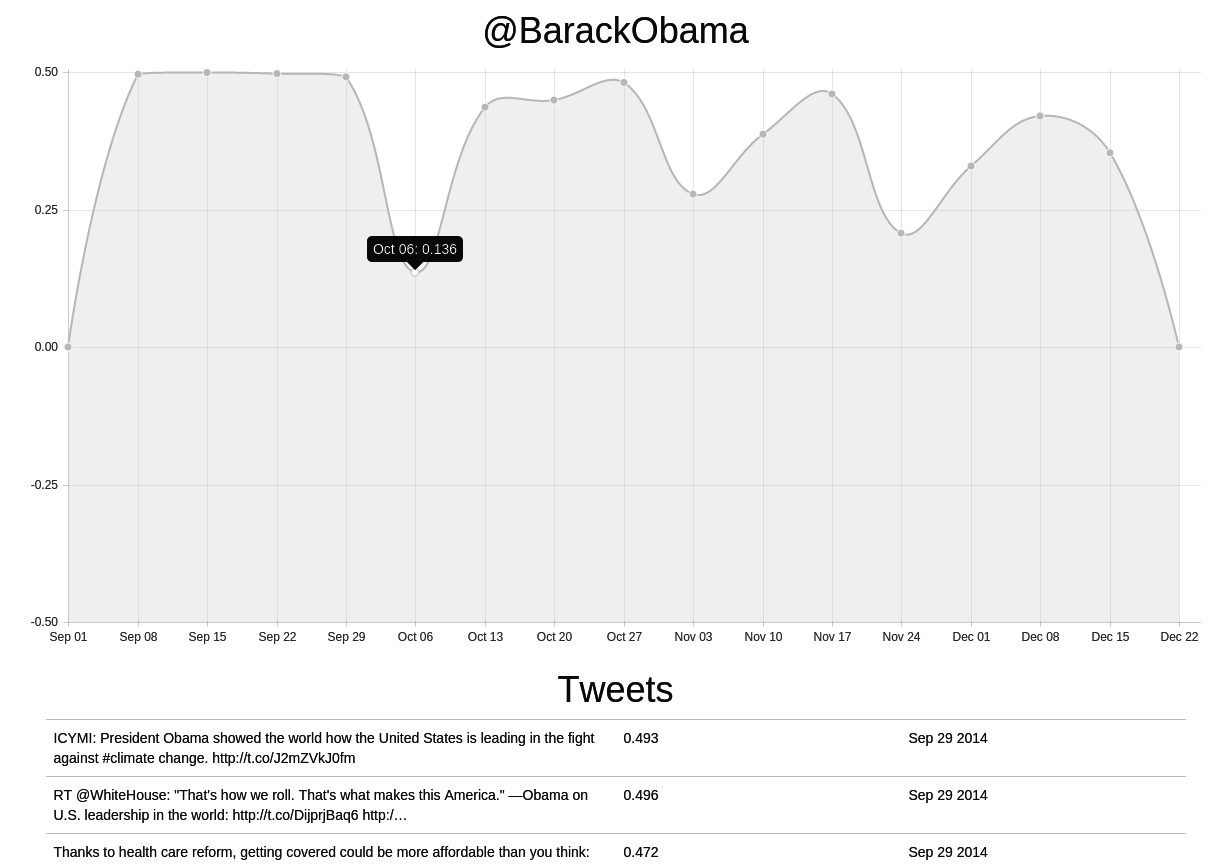
\includegraphics[width=0.8\linewidth]{img/obama_example_usage.png}
  \caption{Example Web Application Screenshot for Twitter User @BarackObama}
  \label{fig:obama}
\end{figure}

\section{Conclusions}

Using a standard Bernoulli Naive Bayes classification algorithm on the largest
500,000 tweet dataset (350,000/150,000 train/test split) with relatively simple
feature extraction techniques, the peak accuracy achieved by this
classification system is 79.12\%. This is a surprisingly good result that shows
the efficacy of simple, probabilistic machine learning techniques when applied
to sentiment analysis.

Most notably, the task of sentiment analysis itself is
not a 100\% agreeable problem.  Specifically, Wilson et al. \cite{wilson05}, in
an empirical analysis, identified that when participants were asked to classify
sentences as ``positive'', ``neutral'', or ``negative'', only 82\% similarity
was recorded, not very far above the accuracy level recorded by this
classifier. When neutral tweets are removed, however, Wilson reported that
accuracy increased to $\sim$90\%. An $80\%$ benchmark by a machine, however, is
still quite good, and is comparable to the state-of-the-art work in statistical
sentiment analysis; Pang et al. \cite{pang02} report a maximum accuracy
percentage with a Naive Bayes classifier of 81.0\%.

\paragraph{Ideas for Further Work}

Only a binary classifier built, since the data was binary - work on
subjectivity. This is mitigated somewhat by flask app averages

\begin{thebibliography}{9}

\bibitem{gamallo14}
  Gamallo, P., and Garcia, M. Citius: A Naive-Bayes Strategy for Sentiment
  Analysis on English Tweets. In \emph{Proceedings of the 8th International
  Workshop on Semantic Evaluation} (Dublin, Ireland, 2014), 171--175.

\bibitem{go09}
  Go, A., Bhayani, R.,  and Huang, L. Twitter Sentiment Classification using
  Distance Supervision. In \emph{Processing} (2009), 1--6.

\bibitem{huang03}
  Huang, J., Lu, J., and Ling, C. X. Comparing Naive Bayes, Decision Trees, and
  SVM with AUC and Accuracy. In \emph{The Third IEEE International Conference
  on Data Mining} (Melbourne, FL, 2003), 553--556.

\bibitem{narayanan13}
  Narayanan, V., Arora, I., and Bhatia, A. Fast and accurate sentiment
  classification using an enhanced Naive Bayes model. In \emph{Intelligent Data
  Engineering and Automated Learning Lecture Notes in Computer Science} (2013),
  194--201.

\bibitem{pak10}
  Pak, A., and Paroubek, P. Twitter as a Corpus for Sentiment Analysis and
  Opinion Mining. In \emph{LREC} (Valletta, Malta, 2010), European Language
  Resources Association, 1320--1326.

\bibitem{pang02}
  Pang, B., Lee, L., and Vaithyanathan, S.
  Thumbs up? Sentiment Classification using Machine Learning Techniques.
  in \emph{Proceedings of EMNLP} (Philadelphia, PA, 2002), Association for
  Computational Linguistics, 79--86.

\bibitem{rennie01}
  Rennie, J. Improving Multi-class Text Classification with Naive Bayes.
  Master's Dissertation (Cambridge, MA, 2001), Massachusetts Institute of
  Technology.

\bibitem{turney02}
  Turney, P.
  Thumbs Up or Thumbs Down? Semantic Orientation Applied to
  Unsupervised Classification of Reviews.
  in \emph{Proceedings of the 40th Annual Meeting of the Association for
  Computational Linguistics} (Stroudsburg, PA, 2002), Association for
  Computational Linguistics, 417--424.

\bibitem{wilson05}
  Wilson, T., Wiebe, J., and Hoffman, P. Recognizing Contextual Polarity in
  Phrase-Level Sentiment Analysis. In \emph{Proceedings of HLT/EMNLP} (2005),
  Association for Computational Linguistics, 347--354.

\end{thebibliography}

\end{document}
